{
\setlength{\belowcaptionskip}{-10pt} 
\begin{table}
{%\footnotesize
\sffamily\small % tabular data either 10pt times, or 9pt helvetica
\centering
\begin{tabular}{|@{\ }l@{\ }||@{\ }c@{\ }|@{\ }c@{\ }|@{\ }c@{\ }|@{\ }c@{\ }|@{\ }c@{\ }|@{\ }c@{\ }||@{\ }r@{\ }|}
  \hline
  \textbf{Program} &  
  {Libs} & {Conc} & {Acts} &
  {Stab} & {Main} & \textbf{Total}
  & \textbf{Build~~~}   
  \\ \hline \hline 
  CAS-lock & 63 & 291 & 509 & 358 & 27 & 1248 & 1m~~~1s
  \\
  Ticketed lock & 58 & 310 & 706 & 457 & 116 & 1647 & 2m~46s
  \\
  CG increment & 26 & - & - & - & 44 & 70 & 8s
  \\
  CG allocator & 82 & - & - & - & 192 & 274 & 14s
  \\
  Pair snapshot & 167 & 233 & 107 & 80 & 51 & 638 & 4m~~~7s 
  \\
  Treiber stack & 56 & 323 & 313 & 133  & 155 & 980 & 2m~41s
  \\
  Spanning tree & 348 & 215 & 162 & 217 & 305 & 1247 & 1m~11s
  \\
  Flat combiner & 92 & 442 & 672 & 538 & 281 & 2025 &  10m~55s
  \\ 
  Seq. stack & 65 & - & - & - & 125 & 190 & 1m~21s
  \\
  FC-stack & 50 & - & - & - & 114 & 164 & 44s
  \\
  Prod/Cons & 365 & - & - & - & 243 & 608 & 2m~43s
  \\[2pt] \hline
\end{tabular}
%\vspace{-5pt}
\caption{
  Statistics for implemented programs: lines of code for program-specific libraries \intab{Libs},
  definitions of concurroids and decorations \intab{Conc}, actions \intab{Acts},
  stability-related lemmas \intab{Stab}, spec and proof sizes of the main
  functions \intab{Main}, total LOC count~\intab{\textbf{Total}}, and build
  times \intab{\textbf{Build}}. The ``\texttt{-}'' entries indicate the
  components that were not needed for the example.
} 
\label{tab:locs}
}
\end{table}}

\section{Evaluation and Experience}
\label{sec:eval-exper}

%
The Coq proof assistant serves as a tool for implementing FCSL's
metatheory and as a language for writing and verifying concurrent
programs.
%
The formalization of the metatheory, which includes the semantic
model, implementation of getters, structural lemmas and a number of
useful libraries (\eg, theory of PCMs, heaps, arrays, \etc.),
is about 17.2 KLOC size.

We evaluated FCSL by implementing, specifying and verifying a number
of characteristic concurrent programs and structures. The simplest
fine-grained structure is a lock, and we implemented two different
locking protocols: CAS-based spinlock and a ticketed
lock~\cite{DinsdaleYoung-al:ECOOP10}. Both locks instantiate a uniform
abstract lock interface, and are used by coarse-grained programs,
performing concurrent incrementation of a pointer and memory
allocation. In addition to the spanning tree algorithm and the flat
combining construction, we also implemented such fine-grained programs
as an atomic pair snapshot~\cite{Qadeer-al:TR09,Liang-Feng:PLDI13} and
non-blocking stack~\cite{Treiber:TR}, both given specs via a PCM of
time-stamped action histories~\cite{Sergey-al:ESOP15} in the spirit of
linearizability~\cite{Herlihy-Wing:TOPLAS90}, as well as several
client programs: a sequential stack (obtained from Treiber stack via
hiding), FC-based stack, and a Treiber stack-based concurrent
Producer/Consumer.

The PCMs employed in formalizations of the case studies are:
%
disjoint sets~\cite{Nanevski-al:ESOP14} (spanning tree, FC, ticketed
lock),
%
heaps~\cite{LeyWild-Nanevski:POPL13} (thread-local
state),
%
natural numbers with addition and zero~\cite{LeyWild-Nanevski:POPL13}
(CG increment),
%
mutual exclusion PCM~\cite{LeyWild-Nanevski:POPL13,Nanevski-al:ESOP14}
(CAS-lock, FC),
%
time-stamped histories~\cite{Sergey-al:ESOP15} (pair snapshot, Treiber
stack, producer/consumer),
%
client-provided PCMs~\cite{LeyWild-Nanevski:POPL13,Nanevski-al:ESOP14}
(FC, locks),
%
\emph{lifted} PCMs---products of basic
PCMs~\cite{LeyWild-Nanevski:POPL13,Nanevski-al:ESOP14} (FC, locks).
%
All these PCM instances are treated uniformly in the proofs
conducted in FCSL, due to the unifying algebraic structure.


%\citeyearpar{Treiber:TR}

Table~\ref{tab:locs} presents some statistics \wrt implemented
programs in terms of LOCs and build times.  The program suite was
compiled on a 2.7 GHz Intel Core i7 OS X machine with 8~Gb RAM, using
Coq~8.4pl4 and Ssreflect~1.4.
%
We didn't rely on any advanced proof automation in the proof scripts,
which would, probably, decrease line counts at the expense of
increased compilation times. Notably, for those programs that required
implementing new primitive concurroids (\eg, locks or Treiber stack),
a large fraction of an implementation is due to proofs of properties
of transitions and actions, as well as stability-related lemmas, while
the sizes of proofs of the main programs' specs are always relatively
small.

{
\setlength{\belowcaptionskip}{-10pt}  
\begin{figure}[t!]
\centering
\ifdefined\psflag
    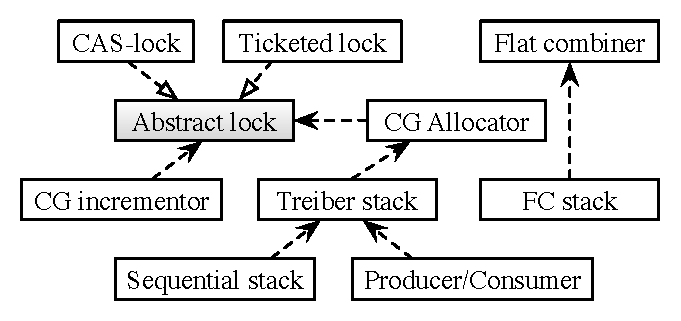
\includegraphics[width=0.45\textwidth]{dependencies.eps}
\else 
    \includegraphics[width=0.45\textwidth]{dependencies-eps-converted-to.pdf}
\fi
%\vspace{-5pt}       
\caption{Dependencies between concurrent libraries.}
\label{fig:deps}
\end{figure}
}
%
Our development is inherently compositional, as illustrated by the
dependency diagram on Figure~\ref{fig:deps}. For example, both lock
implementations are instances of the abstract lock interface,
%
% in the spirit of concurrent abstract
% predicates~\cite{DinsdaleYoung-al:ECOOP10}, 
%
which is used to implement and verify the allocator, which is then
employed by a Treiber stack, used as a basis for sequential stack
and producer/consumer implementations. In principle, we could
implement an abstract interface for stacks, too, to unify the Treiber
stack and the FC-stack, although, we didn't carry out this exercise.

As hinted by Table~\ref{tab:locs}, not every concurrent program
requires implementing a new primitive concurroid: typically this is
done only for libraries, so library clients can reason out of the
specifications.  Table~\ref{tab:concur} shows that the reuse of
concurroids is quite high, and most of the programs make consistent
use of the concurroid for thread-local state and locks (abstracted
through the corresponding interface), as well as of those required by
the used libraries (\eg, Treiber stack or Flat combiner).
%
